\section{Automatic Movement Overhaul}\label{sec:automatic-movement-overhaul}

As pointed out in section~\ref{subsec:problems-with-automatic-movement}, the current automatic movement method was
built as temporary means to navigate between saved bookmarks.
The method applies a linear interpolation to transition smoothly between the origin and target position leading to
movement in a straight line between the two points.
Additionally, a linear interpolation between the origin and target orientation is used to rotate the observer into the
target orientation.
\\
While this is the easiest, and most straightforward way to smoothly move the observer through the simulation without
breaking continuity by teleporting the user, the simultaneous translation and rotation have been found to induce
disorientation followed up by motion sickness symptoms by the user.
\\
\\
In this section a new automatic navigation for CosmoScout is presented, which aims to make the automatic navigation
more accessible and less sickness inducing.
As parts of the navigation have not been fully implemented, we first present the concepts how the automatic
navigation system should move the observer.
After the concept, key features of the implemented solutions are presented and explained.


\subsection{Automatic Movement Concept}\label{subsec:automatic-movement-concept}

The main goal, found to reduce cybersickness for automatic movement, is reducing the complexity of the movement by
decoupling the rotation from the translation.
This way the movements are easier to read, and the user should be able to better anticipate the observers movements,
reducing motion sickness symptoms.
\\
First, the linear interpolation is exchanged for movement along a spline.
This way, it does not change the linear movement between points in space as it was implemented before, while still
accomodating for different, non-linear paths the observer can take.
Additionally, this change is made to facilitate more variability for later development, like programmed virtual tours
along points of interest.
Additionally, the change to splines is made to enable easier collision handling for the navigation method, as
additional control points can be inserted to handle collisions and divert the movement path.
\\
\\
Since the origin and target location and orientation of the automatic navigation can be arbitrary points anywhere in
the simulation (both bookmarked and calculated intermediate locations), the first step is to classify the possible
locations into groups.
We propose the classification of locations based on their location relative to other bodies, and the SPICE reference
frame the location is in:
\begin{itemize}
    \item Surface locations, that are close to, or on the surface of a body, where the location's position and
    orientation are in the respective body's SPICE frame relative to the body's center;
    \item Orbit locations, where the location is not on or close to the surface, but the position and orientation
    are still relative to the body's SPICE frame and center;
    \item Interplanetary locations, where the location's position and orientation is not relative to another body's
    SPICE frame and center, but the solar system's barycenter, i.e.\ the "J2000" SPICE frame.
\end{itemize}
Through the classification of locations a set of general movements and transitions can be derived to access all of
those locations in a manner that is predictable for the user, while still general enough to minimize special cases
that could lead to unwanted behaviour.
\\
The classification leads to 3 types of movement and the transitions between them, as shown in table~\ref{tab:auto-move-types}:
\begin{center}
    \begin{tabular}{c | c c c}
        \toprule
        \textbf{Origin \textbackslash Target} & \textbf{Surface} & \textbf{Orbit} & \textbf{Interplanetary}\\
        \midrule
        \textbf{Surface}         & Surface movement & Surface to Orbit transition & - \\
                                 &                  & (Ascending)                 &   \\
        \textbf{Orbit}           & Orbit to Surface transition & Orbital movement & Orbital transition \\
                                 & (Descending)                &                  &                    \\
        \textbf{Interplanetary}  & - & - & Interplanetary movement \\
        \bottomrule
    \end{tabular}
    \captionof{table}{Possible movement and transition types for the automatic navigation.}
    \label{tab:auto-move-types}
\end{center}
the different movements are structured in layers, therefore a transition from surface to interplanetary space and
vice versa is done via transition from surface to orbit, and from orbit to interplanetary space.
Additionally, there is no transition from interplanetary movement to orbital movement since the interplanetary
movements end in a position where no further transition is needed.
\\
An example for this layered travel is a movement from a location on the origin body's surface to a location on the
target body's surface:
First, the observer transitions from the surface location to an orbit location via an ascending transition.
In orbit, the observer transitions to a position to facilitate interplanetary movement, and moves to the target
body into an orbit position.
Then, an orbital movement is performed to move above the final location on the surface.
Finally, the observer transitions to the final location on the surface via a descending transition.

\subsubsection{Surface Movement}\label{subsubsec:surface-movements}

\begin{wrapfigure}{o}{0.25\textwidth}
    \centering
    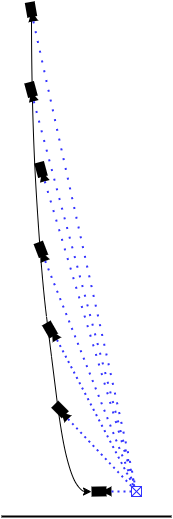
\includegraphics[width=0.1\textwidth]{content/4_3_autoNavigation/img/PlannedLanding}
    \caption{Planned automatic movement descending onto a body's surface.}
    \label{fig:new-auto-nav-descend}
\end{wrapfigure}
In this overhaul, we did not primarily focus on a solution for automatic movement on the surface of a body, since
those movements are strongly dependent on distance and topology between the target and origin.
Additionally, surface navigation is difficult to test under the current circumstances, since a connection to the DLR
map server is needed to poll street level elevation data and textures, and both were unavailable in the remote work
setting due to the COVID-19 pandemic.
\\
In order to find a general solution, independent of distance and topology, we chose to facilitate surface movements
via orbital travel, i.e.\ transitioning from the surface origin location into orbit, using orbital movement to go to an
orbital location above the target surface location and transitioning back down to the surface at the target location.
\\
While this solution may be inconvenient for short distances relative to the body's circumference, we assume this form
of movement to be a default solution independent of topology or distance.
Further solutions for surface movements, especially for short distances, should be easily implementable in later
works using the established framework we develop here.
\\
\\
The important changes in the surface movement are the transitions between surface and orbit (the landing and
ascending movements).
\\
In order to prevent the change of reference frame, as pointed out in
section~\ref{subsec:problems-with-automatic-movement}, we plan to change the linear path and simultaneous rotation
shown in figure~\ref{fig:old-auto-nav-descend}, to a parabolic curve, so the observer's movements are always
perceived as forward, not downward, and the observer swoops into the target location on the surface, as depicted in
figure~\ref{fig:new-auto-nav-descend}.
\\
To ease the rotation and enable the user to predict the movement, the center of the viewport is aimed at a point
slightly in front of the final position in direction of the final orientation.
This essentially separates the translation from the rotation due to the steepness of the movement.
The bulk of the rotation during the movement is at the end of the curve where the curvature is highest.
\\
\\
The ascending transition is basically similar, but in reverse, so the observer zooms out moving backwards and
focusing on the point of origin until it reaches the default orbital distance where the point of origin should almost
coincide with the body's center.

\subsubsection{Orbital Movement}\label{subsubsec:orbital-movements}

The default orbital distance for each body is relative to the body size, so that the orbited body always occupies the
same space of the viewport, independent of the body's size.
In order to prevent movements through the body as shown in figure~\ref{fig:old-auto-nav-collision} in
section~\ref{subsec:problems-with-automatic-movement}, we plan to use the flexibility of splines to move the observer
in circular curves around the body, while focusing the center of the viewport on the center of the body.
\\
While this movement has simultaneous translation and rotation, this movement is not perceived by most users as the
observer moving around the body, but a rotation of the whole simulation around the body where the viewport is focused
on.
In case either the starting point, or the final location are not equidistant to the boday's center, the curve becomes
less circular, but the nature of the spline should compensate for different distances to the center automatically,
leading to the user perceiving the change in distance as the observer zooming out, away from the body during the
rotation.
\\
\\
For the transition from orbital to interplanetary movement, a few steps are added to reduce surprising rotations and
make the movement easier to predict by the user.
\begin{figure}[h]
    \centering
    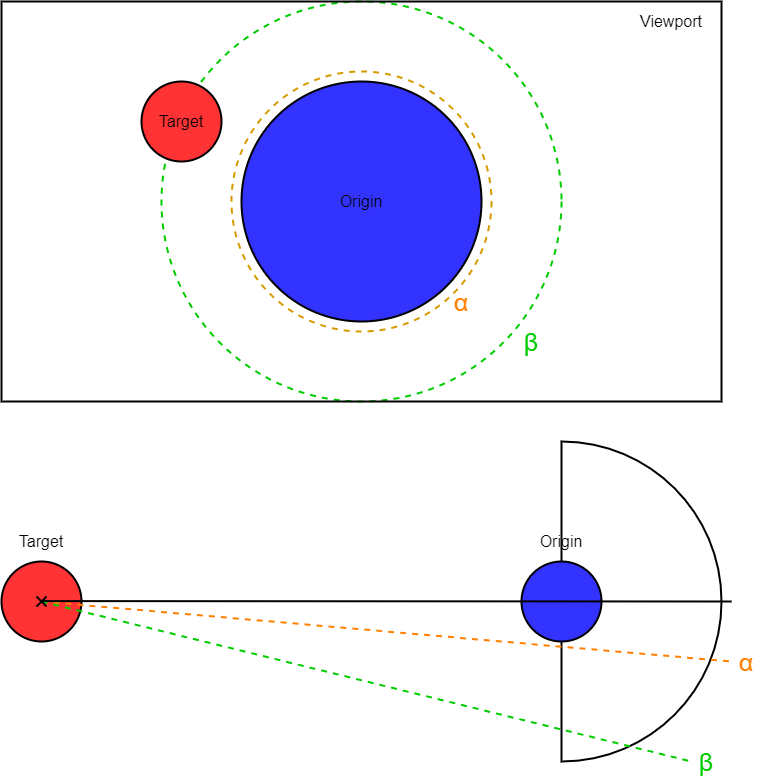
\includegraphics[width=0.66\textwidth]{content/4_3_autoNavigation/img/OrbitTransitionAngles}
    \caption{Minimum ($\alpha$) and maximum ($\beta$) angle for the transition into interplanetary movement.}
    \label{fig:orbital-transition-angles}
\end{figure}
First, the observer finds the closest suitable location where the following conditions are met:
\begin{itemize}
    \item The angle $\theta$ between the vector from the target's center to the observer, and the vector from the
    target's center to the origin's center is between the minimum allowed angle $\alpha$ and the maximum allowed
    angle $\beta$.
    \begin{equation}
        \label{eq:orbital-angles}
        \alpha >= \theta >= \beta
    \end{equation}

    \item The vector $\vec{v}$ between the target's center, and the observer must be longer than the vector $\vec{w}$
    between the target's center, and the origin's center.
    \begin{equation}
        \label{eq:orbital-magnitudes}
        |\vec{v}| > |\vec{w}|
    \end{equation}
\end{itemize}
\\
The requirements are visualised in figure~\ref{fig:orbital-transition-angles}.
The first requirement (equation~\ref{eq:orbital-angles}), creates two cones from the target's center towards the origin.
The $\alpha$-cone is the minimum angle, that prevents the target from being mostly obscured by the origin body, and
the $\beta$-cone is the maximum angle, that ensures the Target is still visible on the viewport.
Both cones intersect the sphere of the origin's possible orbit locations twice, resulting in two spherical segments.
\\
The second requirement excludes the spherical segment that is in between the origin and target bodies.
The spherical zone of the remaining segment are the available locations for the interplanetary transitions,
figure~\ref{fig:orbital-transition-zone} visualises the possible locations.
\begin{wrapfigure}{o}{0.25\textwidth}
    \centering
    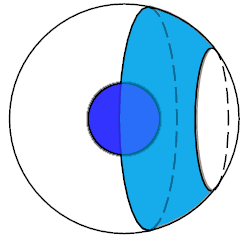
\includegraphics[width=0.2\textwidth]{content/4_3_autoNavigation/img/OrbitTransitionSphericalZone}
    \caption{Spherical zone of locations available for the interplanetary transition.}
    \label{fig:orbital-transition-zone}
\end{wrapfigure}
\\
The transition for interplanetary movement is to move to the closest location in this spherical zone via orbital
movement, which results in a scene similar to the viewport in figure~\ref{fig:orbital-transition-angles}, where the
viewport is focused on the center of the origin's body, and the target body is within the $\alpha$ and $\beta$
margins in the viewport.

\subsubsection{Interplanetary Movement}\label{subsubsec:interplanetary-movement}

The interplanetary movement remains closest to the original movement.
However, the interpolation between the origin and target orientation is removed in order to separate rotation from
translation and increase predictability.
Instead, the rotation is split into an initial rotation to fave the traveling direction, so the user always moves
forward, towards the target, and a final rotation at the end of the translation to rotate the observer into the final
orientation at the target location.
\\
The translation uses a straight spline.
This way the movement is similar to the original interpolation between the origin and target position.
However, the spline allows easier modification of the path, leading to easier collision detection and mitigation in
the future, since the spline can be easily checked for collisions and, if necessary, additional control points can be
inserted into the spline to avoid collisions.
The interplanetary movement always ends in either an interplanetary location (bookmark) or a target body's orbit,
where orbital movement can be resumed.
Therefore, no transition from interplanetary movement to orbital movement is needed.
\\
\\
\begin{figure}[h]
    \centering
    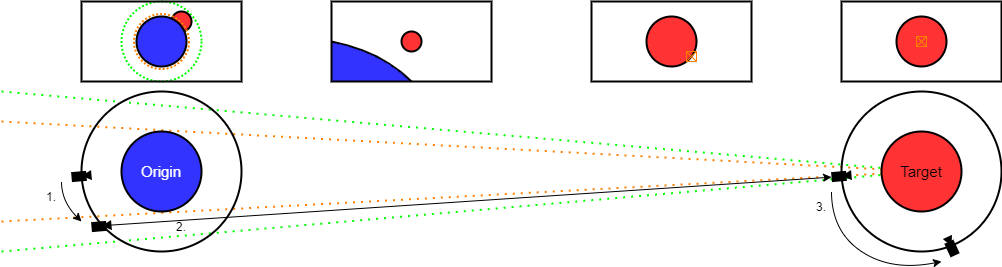
\includegraphics[width=\textwidth]{content/4_3_autoNavigation/img/Orbit2OrbitExample}
    \caption{Example of automatic movement including the orbital to interplanetary movement transition (1.), the
    interplanetary movement (2.), and orbital movement the the final position (3.).}
    \label{fig:orbital-example}
\end{figure}
An example of movement between two orbital locations, is shown in figure~\ref{fig:orbital-example}.
\\
The first step shown in the figure is the transition from an arbitrary orbital location around the origin body to a
location that fulfills the requirements (equations~\ref{eq:orbital-angles}~\&~\ref{eq:orbital-magnitudes}).
\\
The second step is the interplanetary movement between the origin orbit, and the target orbit.
First, the observer rotates from focusing on the origin's center to the target's center, and travel direction.
During this rotation the requirements for the transition between orbital and interplanetary movement, help reduce the
angular distance of the rotation and prevent collision with the origin body during interplanetary travel.
\\
After arriving at the target's orbit, the third step is an orbital movement to the final position.
\\
\\
While this staged approach increases the overall travel time of the automatic navigation, we aim to reduce
disorientation and resulting cybersickness symptoms by providing the user with an easily predictable solution that
decouples rotation from translation and minimizes complex and surprising rotations.



\subsection{Automatic Movement Implementation}\label{subsec:automatic-movement-implementation}
